% Thesis chapter: simulation study comparing heuristic, RL, BC, and BC->RL.
% Standalone chapter file; \input or \include from the thesis root.
% Distills the IROS draft results with the stability-metric caveat applied:
% stability numbers from this campaign (overdamped passive chain) are not
% reported, and no stability-improvement claim is made.

\chapter{Learning to Clear Piles in Simulation}
\label{ch:sim_study}

This chapter asks the first question of the thesis: can a policy learn
sequential grasp targeting for dense piles from raw point clouds, and what
combination of learning methods gets it there? Four methods are compared on
the testbed of Chapter~\ref{ch:sim_env} under one shared controller, pile
distribution, and evaluation protocol: the privileged heuristic expert,
reinforcement learning from scratch, behavior cloning of the expert, and
behavior cloning followed by reinforcement learning fine-tuning. The result
that organizes everything downstream is a clean dissociation: from-scratch RL
fails at the trajectory level regardless of what it observes, behavior
cloning from raw clouds reaches near-expert clearing, and a carefully
constrained fine-tuning recipe preserves that competence while optimizing
per-grasp execution.

\section{Behavior Cloning}
\label{sec:study_bc}

Demonstrations are collected by running the privileged expert of
Section~\ref{sec:sim_expert} and recording, for each successful grasp, the
point cloud observation and the expert action encoded in the policy's action
space (positions through the inverse squashing map, yaw as the doubled-angle
pair). Failed grasps are discarded. The dataset used here contains roughly
20{,}700 successful-grasp samples with an 85/15 train/validation split.

The policy is a PointNet encoder~\cite{qi2017pointnet} followed by a small
actor head. A shared per-point multilayer perceptron
($3 \to 64 \to 128 \to 256$, batch normalization, ELU
activations~\cite{clevert2015elu}) maps each point independently; a
channelwise max-pool aggregates the set; a fully connected layer produces a
256-dimensional global feature; and an actor MLP
($256 \to 128 \to 64 \to 5$) with dropout 0.2 outputs the action. Training
minimizes mean-squared error against the expert action with
AdamW~\cite{loshchilov2019adamw} (learning rate $10^{-4}$, weight decay
$10^{-4}$), plateau scheduling, and early stopping on validation loss. For
the privileged-pose ablation the encoder is replaced by an MLP on the
128-dimensional pose vector.

\section{Reinforcement Learning from Scratch}
\label{sec:study_rl}

The RL baselines are trained with proximal policy
optimization~\cite{schulman2017ppo} in the RSL-RL
library~\cite{schwarke2025rslrl}, using a Gaussian policy over the same 5D
action space and a symmetric actor-critic: actor and critic each process the
observation through their own encoder (PointNet for cloud inputs, MLPs for
the pose ablation), so the value gradient doubles as an auxiliary
representation-learning signal. The reward is the per-cycle outcome product
\begin{equation}
  r = n \cdot \alpha \cdot \varsigma
  \label{eq:study_reward}
\end{equation}
for successful grasps and $r = -1$ for failures, where $n$, $\alpha$, and
$\varsigma$ are the throughput, alignment, and stability scores of
Section~\ref{sec:sim_outcome}. The reward is entirely per-grasp: any
trajectory-level clearing competence must emerge from targeting strategy
rather than from explicit shaping. Key settings: initial policy standard
deviation $\sigma_0 = 1.0$, clip 0.2, entropy coefficient 0.01, learning rate
$3 \times 10^{-4}$ with adaptive KL scheduling (target 0.01), generalized
advantage estimation ($\lambda = 0.95$), and discount $\gamma = 0.99$.

\section{BC-Initialized Fine-Tuning}
\label{sec:study_bcrl}

The fine-tuned policy loads the trained BC actor (encoder and head) into the
PPO actor and continues training on-policy~\cite{rajeswaran2018learning,
nair2018overcoming}, with three deliberate constraints
(Figure~\ref{fig:study_pipeline}).

First, the critic is \emph{asymmetric}~\cite{pinto2018asymmetric}: it is a
freshly initialized MLP on the privileged 128-dimensional pose state rather
than on the point cloud. It learns an accurate value function within a few
iterations, precisely because it does not need to learn perception, and it
shares no parameters with the actor.

Second, the BC-trained PointNet encoder is \emph{frozen}. The state-based
critic cannot propagate gradients through the visual pathway, so an unfrozen
encoder would drift without constraint; in practice, fine-tuning the full
network collapses training (Figure~\ref{fig:study_ablation}).

Third, exploration starts \emph{small}: $\sigma_0 = 0.05$ instead of 1.0,
restricting early rollouts to small perturbations around the BC policy's
actions. Higher noise degrades the initialization faster than reward feedback
can compensate, gradually at $\sigma_0 = 0.1$ and rapidly at
$\sigma_0 = 0.3$ (Figure~\ref{fig:study_ablation}). All other
hyperparameters match the from-scratch configuration. Because return degrades
late in long fine-tunes, the evaluation checkpoint is selected by early
stopping.

\begin{figure}[t]
\centering
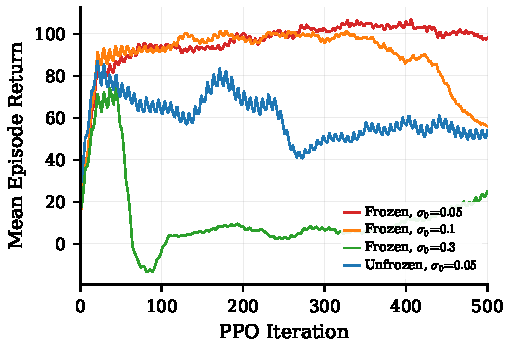
\includegraphics[width=\linewidth]{bcrl_ablation_minimal.pdf}
\caption{Fine-tuning sensitivity. Mean episode return against PPO iteration
for four configurations varying encoder freezing and initial exploration
noise $\sigma_0$. Only the frozen-encoder, $\sigma_0 = 0.05$ configuration
sustains performance; unfreezing the encoder collapses training regardless of
noise level, and larger $\sigma_0$ degrades the BC initialization gradually
(0.1) or rapidly (0.3).}
\label{fig:study_ablation}
\end{figure}

\begin{figure}[t]
\centering
\resizebox{\linewidth}{!}{%
\begin{tikzpicture}[
  block/.style={rectangle, rounded corners=3pt, draw=black!70,
    text width=3.0cm, minimum height=0.7cm, align=center,
    font=\scriptsize, inner sep=4pt},
  frozen/.style={block, fill=blue!12},
  trainable/.style={block, fill=orange!18},
  io/.style={block, fill=white},
  lossnode/.style={rectangle, rounded corners=3pt, draw=black!50, dashed,
    text width=3.4cm, align=center, font=\scriptsize, inner sep=4pt, fill=gray!5},
  wideloss/.style={lossnode, text width=5.5cm},
  arr/.style={-{Stealth[length=4pt]}, thick, black!70},
  panelbg/.style={rectangle, rounded corners=6pt, draw=gray!50,
    fill=gray!3, inner sep=8pt},
  ptitle/.style={font=\small\bfseries},
  collabel/.style={font=\scriptsize\itshape, text=black!60},
]
% ====== PANEL (a): BEHAVIOR CLONING ======
\node[io] (a_pcd) at (0, 0)
  {Raw cloud\\$P_t \in \mathbb{R}^{1024\times3}$};
\node[io] (a_expert) at (4, 0)
  {Expert heuristic\\$a^{*} \in \mathbb{R}^{5}$};
\node[trainable, below=0.25cm of a_pcd] (a_enc)
  {PointNet encoder\\$3\!\to\!64\!\to\!128\!\to\!256$\\BN + ELU, max-pool\\$\to\mathbb{R}^{256}$};
\node[trainable, below=0.25cm of a_enc] (a_mlp)
  {Actor MLP\\$256\!\to\!128\!\to\!64\!\to\!5$\\ELU, dropout$\!=\!0.2$};
\node[lossnode, below=0.25cm of a_mlp] (a_loss)
  {$\mathcal{L}_{\text{BC}} = \lVert\mu_\theta(\mathbf{z}) - a^{*}\rVert^{2}$};
\draw[arr] (a_pcd) -- (a_enc);
\draw[arr] (a_enc) -- (a_mlp);
\draw[arr] (a_mlp) -- (a_loss);
\draw[arr] (a_expert.south) |- (a_loss.east);
%
% ====== PANEL (b): RL FINE-TUNING ======
\node[collabel] (b_alabel) at (8.5, 0.55) {Actor (vision)};
\node[collabel] (b_clabel) at (12.5, 0.55) {Critic (privileged)};
\node[io] (b_pcd) at (8.5, 0) {Raw cloud\\$P_t \in \mathbb{R}^{1024\times3}$};
\node[frozen, below=0.25cm of b_pcd] (b_enc)
  {PointNet encoder\\(from BC, frozen)\\$3\!\to\!64\!\to\!128\!\to\!256$\\$\to\mathbb{R}^{256}$};
\node[trainable, below=0.25cm of b_enc] (b_actor)
  {Actor MLP\\(init from BC)\\$256\!\to\!128\!\to\!64\!\to\!5$\\ELU};
\node[trainable, below=0.25cm of b_actor] (b_policy)
  {$\pi = \mathcal{N}(\mu, \sigma^{2} I)$\\$\sigma_0 = 0.05$};
\node[io] (b_state) at (12.5, 0)
  {Privileged state\\$\xi_t \in \mathbb{R}^{128}$};
\node[trainable, below=0.25cm of b_state] (b_cenc)
  {Critic encoder\\$128\!\to\!256\!\to\!256$\\ELU};
\node[trainable, below=0.25cm of b_cenc] (b_cmlp)
  {Critic MLP\\$256\!\to\!128\!\to\!64\!\to\!1$\\ELU};
\path (b_policy.south) ++(0,-0.5) coordinate (ppo_y);
\path (b_pcd.center) -- (b_state.center) coordinate[midway] (ppo_x);
\node[wideloss] (b_ppo) at (ppo_y -| ppo_x)
  {PPO\enspace $\varepsilon\!=\!0.2,\;\gamma\!=\!0.99,\;\lambda\!=\!0.95$};
\draw[arr] (b_pcd) -- (b_enc);
\draw[arr] (b_enc) -- (b_actor);
\draw[arr] (b_actor) -- (b_policy);
\draw[arr] (b_state) -- (b_cenc);
\draw[arr] (b_cenc) -- (b_cmlp);
\draw[arr] (b_policy.south) -- (b_policy |- b_ppo.north);
\draw[arr] (b_cmlp.south) -- (b_cmlp |- b_ppo.north);
%
% ====== PANEL (c): INFERENCE ======
\node[io] (c_pcd) at (17, 0) {Raw cloud\\$P_t \in \mathbb{R}^{1024\times3}$};
\node[frozen, below=0.25cm of c_pcd] (c_enc)
  {PointNet encoder\\(from BC)\\$\to\mathbb{R}^{256}$};
\node[frozen, below=0.25cm of c_enc] (c_actor)
  {Actor MLP\\(from RL)\\$\mu_\theta(\mathbf{z}) \in \mathbb{R}^{5}$};
\node[io, below=0.25cm of c_actor] (c_scale)
  {tanh + scale\\$\to(x,y,z,\psi)$};
\node[io, below=0.25cm of c_scale] (c_fsm) {FSM controller};
\draw[arr] (c_pcd) -- (c_enc);
\draw[arr] (c_enc) -- (c_actor);
\draw[arr] (c_actor) -- (c_scale);
\draw[arr] (c_scale) -- (c_fsm);
%
\begin{scope}[on background layer]
  \node[panelbg, fit=(a_pcd)(a_expert)(a_enc)(a_mlp)(a_loss)] (bg_a) {};
  \node[panelbg, fit=(b_alabel)(b_clabel)(b_pcd)(b_enc)(b_actor)(b_policy)(b_state)(b_cenc)(b_cmlp)(b_ppo)] (bg_b) {};
  \node[panelbg, fit=(c_pcd)(c_enc)(c_actor)(c_scale)(c_fsm)] (bg_c) {};
\end{scope}
\node[ptitle, above=2pt of bg_a.north] {(a) Behavior cloning};
\node[ptitle, above=2pt of bg_b.north] {(b) RL fine-tuning};
\node[ptitle, above=2pt of bg_c.north] {(c) Inference};
%
\draw[-{Stealth[length=6pt]}, very thick, gray!50]
  (bg_a.east |- bg_b.west) -- (bg_b.west);
\draw[-{Stealth[length=6pt]}, very thick, gray!50]
  (bg_b.east) -- (bg_c.west |- bg_b.east);
%
\coordinate (leg_start) at ($(bg_a.center |- b_ppo) + (-3.0, 0)$);
\node[rectangle, rounded corners=2pt, draw=black!70, fill=orange!18,
  minimum width=0.5cm, minimum height=0.25cm] (leg_t) at (leg_start) {};
\node[font=\scriptsize, right=2pt of leg_t] (leg_tl) {Trainable};
\node[rectangle, rounded corners=2pt, draw=black!70, fill=blue!12,
  minimum width=0.5cm, minimum height=0.25cm, right=0.6cm of leg_tl] (leg_f) {};
\node[font=\scriptsize, right=2pt of leg_f] (leg_fl) {Frozen};
\node[rectangle, rounded corners=2pt, draw=black!50, dashed, fill=gray!5,
  minimum width=0.5cm, minimum height=0.25cm, right=0.6cm of leg_fl] (leg_l) {};
\node[font=\scriptsize, right=2pt of leg_l] {Loss / Optimizer};
\end{tikzpicture}%
}
\caption{The BC-to-RL pipeline. (a)~The PointNet encoder and actor MLP are
trained end-to-end on expert demonstrations with an MSE loss. (b)~The encoder
is frozen and the actor MLP is fine-tuned with PPO alongside a state-based
asymmetric critic. (c)~At inference the critic is discarded; the encoder and
actor run deterministically through the FSM.}
\label{fig:study_pipeline}
\end{figure}

\section{Evaluation Protocol}
\label{sec:study_protocol}

Each method is evaluated over 100 episodes on 200-log piles, distributed
across 20 parallel environments, with identical random seeds across methods
so that every policy faces the same pile configurations. Metrics are
per-episode means with standard deviations. Training used 20 parallel
environments for point cloud policies and 32 for pose-based policies on a
single RTX 4070 Laptop GPU (8~GB), which bounds the practical model and batch
sizes and is worth stating because the entire pipeline is reproducible on
laptop-class hardware.

\section{Results}
\label{sec:study_results}

\begin{table}[t]
\centering
\caption{Simulation comparison across 100 episodes on randomized 200-log
piles (mean $\pm$ std). All methods share the controller and evaluation
seeds. The heuristic reads privileged pose state; RL variants use a symmetric
actor-critic; BC$\to$RL uses the frozen-encoder asymmetric recipe of
Section~\ref{sec:study_bcrl}. Stability is excluded from this campaign's
reporting (Section~\ref{sec:sim_study_stability}).}
\label{tab:study_results}
\small
\setlength{\tabcolsep}{4pt}
\begin{tabular}{llccccc}
\hline
\textbf{Method} & \textbf{Obs.} & $n$ & $\alpha$ & \textbf{Succ.\,(\%)} &
\textbf{Clear\,(\%)} & \textbf{Knocked\,(\%)} \\
\hline
Heuristic & Pose & $9.94 \pm 1.17$ & $0.918 \pm 0.031$ & $88.7 \pm 7.8$ & $99.0 \pm 1.2$ & $1.0 \pm 1.1$ \\
\hline
RL & Pose & $8.84 \pm 1.68$ & $0.908 \pm 0.040$ & $38.5 \pm 13.5$ & $49.4 \pm 14.8$ & $0.0 \pm 0.2$ \\
RL & Seg.\ cloud & $7.04 \pm 1.06$ & $0.726 \pm 0.077$ & $53.7 \pm 10.9$ & $55.2 \pm 5.4$ & $0.9 \pm 0.7$ \\
RL & Raw cloud & $6.78 \pm 1.01$ & $0.758 \pm 0.072$ & $53.3 \pm 8.7$ & $53.0 \pm 3.9$ & $0.6 \pm 0.6$ \\
\hline
BC & Seg.\ cloud & $9.64 \pm 1.05$ & $0.907 \pm 0.028$ & $70.3 \pm 10.6$ & $96.5 \pm 4.7$ & $0.9 \pm 1.0$ \\
BC & Raw cloud & $9.32 \pm 1.12$ & $0.904 \pm 0.037$ & $84.5 \pm 9.8$ & $98.5 \pm 5.1$ & $0.7 \pm 0.7$ \\
\hline
BC$\to$RL & Raw cloud & $8.65 \pm 0.97$ & $0.906 \pm 0.027$ & $86.3 \pm 8.5$ & $98.2 \pm 1.5$ & $1.2 \pm 0.8$ \\
\hline
\end{tabular}
\end{table}

\begin{figure}[t]
\centering
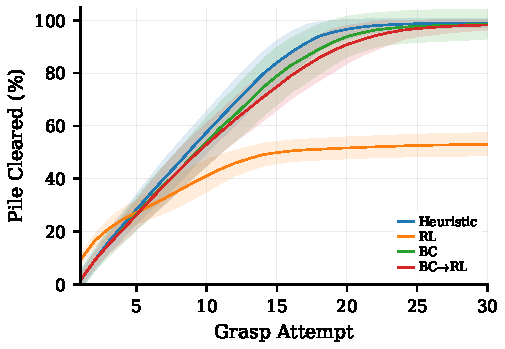
\includegraphics[width=0.9\linewidth]{clearing_curves.pdf}
\caption{Clearing progression: fraction of the 200-log pile cleared against
grasp attempt number (mean $\pm$ std over 100 episodes). From-scratch RL
diverges from the other methods around grasp 5 to 10 and plateaus near half
the pile, while the heuristic, BC, and BC$\to$RL all approach full clearing.}
\label{fig:study_clearing}
\end{figure}

Table~\ref{tab:study_results} and Figure~\ref{fig:study_clearing} summarize
the comparison. Three findings matter.

\subsection{From-scratch RL fails at the trajectory level}

Every from-scratch RL variant plateaus at roughly half the pile (49 to 55\%
clearing) while the heuristic, BC, and the fine-tuned policy all exceed 98\%.
The failure is not perception: the privileged-pose variant, which observes
exact log states, clears no more of the pile than the cloud variants. It is
also not reward design: shaping ablations that simplify the reward to
throughput only (54.2\% clearing) or normalize throughput by available logs
(48.3\%) leave the plateau intact. What remains is exploration. The policies
reach competitive per-grasp reward during training, then the clearing curves
flatten once the easily accessible logs are exhausted: the learned targeting
pattern works in dense configurations and fails to adapt as the pile thins,
and random exploration never visits the sparse endgame states from which it
could learn otherwise. High per-grasp return with low clearing is exactly
the signature of a per-grasp-greedy policy in a sequential task.

\subsection{BC transfers the expert's trajectory coverage}

Behavior cloning on raw clouds reaches $98.5\%$ clearing, statistically
indistinguishable from the privileged expert it imitates, with per-grasp
metrics close behind (largest gap: grasp success, 84.5\% versus 88.7\%). The
demonstrations span complete clearing trajectories from dense stack to empty
rack, handing the policy precisely the state coverage that RL exploration
fails to acquire. Notably, raw clouds match or exceed segmented clouds under
BC (98.5 versus 96.5\% clearing, 84.5 versus 70.3\% success): the encoder
learns to attend to task-relevant geometry without segmentation, and the
simpler pipeline carries no segmentation model whose sim-to-real mismatch
would later need managing.

\subsection{Constrained fine-tuning preserves competence}

The BC$\to$RL policy retains full clearing ($98.2\%$) and the expert-level
success rate while training on task reward, confirming that the
frozen-encoder, low-noise, asymmetric-critic recipe lets on-policy RL run
without destroying the cloned competence; the ablation of
Figure~\ref{fig:study_ablation} shows every relaxation of the recipe
collapsing. Under observation noise the fine-tuned policy degrades more
gracefully than BC (93.9 versus 83.2\% clearing at 0.1~m additive noise, 52.6
versus 31.3\% at 0.2~m), consistent with on-policy training exposing the
policy to its own action-induced state distribution. Throughput dips
slightly (8.65 versus 9.32 logs per successful grasp), the price of
optimizing per-cycle outcome scores that penalize sloppy multi-log bites.

Under pile variation (randomized log count from 20 to 200, grid dimensions,
spacing, layer offsets, and per-log jitter), all three competent methods hold
near-complete clearing (heuristic $98.2\%$, BC $98.4\%$, BC$\to$RL $98.5\%$),
with throughput and success declining for all methods as smaller and
irregular piles offer fewer easy multi-log grasps; the learned policies drop
more in success rate than the heuristic, plausibly because demonstrations
were collected on fixed 200-log piles.

\section{On the Stability Metric}
\label{sec:sim_study_stability}

This campaign also measured the stability score $\varsigma$ of
Equation~\eqref{eq:sim_stability}, and the fine-tuned policy appeared to
improve it substantially over both BC and the heuristic. That result is
deliberately not reported as a finding. The apparent gain was measured under
the passive-chain model with spring-damper values (stiffness 300, damping
500) that later hardware comparison showed to be overdamped: the spring
recenters the suspended grapple and the heavy damping suppresses swing, so
simulated loads ride more level than the real, freely pivoting hanger allows,
and the metric was both inflated and compressed in a regime where small
differences are not physically meaningful. In addition, the single-snapshot
evaluation of the original metric samples the tilt at one instant of the
hold rather than characterizing the settling transient. Both defects were
subsequently fixed, the chain freed (zero stiffness, light damping) and the
metric redefined as a windowed mean tilt with a settling criterion mirroring
the on-crane measurement procedure, and stability comparisons in this thesis
are made only under the corrected model (Chapter~\ref{ch:bcrl}). The
clearing, success, throughput, and alignment results of this chapter are
unaffected: they do not depend on the suspension model in any comparable way,
and the qualitative conclusions (RL's exploration failure, BC's coverage
transfer, the fine-tuning recipe's preservation of competence) stand.

\section{Summary}

At pile scale, the exploration problem dominates: from-scratch RL fails at
roughly half the pile regardless of observation type or reward shaping, while
behavior cloning of a privileged expert transfers full-trajectory competence
from raw, unsegmented point clouds. Fine-tuning the cloned policy with PPO
under a frozen encoder, a privileged asymmetric critic, and conservative
exploration preserves clearing at expert level while optimizing per-grasp
execution, and improves robustness to observation noise. These findings fix
the architecture of everything that follows: imitation supplies perception
and coverage, reinforcement learning refines the decision, and the
deployment-oriented chapters build on exactly this division of labor.
